\chapter{Event Reconstruction \& Simulation} \label{chap-EventReconstruction&Simulation}

Monte Carlo (MC) simulations are an essential part of current particle physics analyses and are used to mimic physical processes that correspond to those which are observed within the LHC, and other such experiments. Analysts compare findings in data to simulation in order to extract signal processes, and also to perform statistical analysis on results obtained. It is of the utmost importance that the simulated events must be as accurate as physically possible in order to mimic real life processes and perform a scientifically accurate analysis. Will talk about methods for generating events, including the different MC generators and tunes used in the evaluation of theoretical uncertainties, and interpretation in terms of the CMS detector in the first section of this chapter.

Roughly speaking, we can divide the different steps of event reconstruction into three separate processes. The first of which records basic information, such as hits within the pixel detectors of the inner tracking system, and calorimeter energy clusters, for `low level' objects in each sub-detector. The information is then passed to the PF algorithm which uses information from all the sub-detectors in order to reconstruct events much more accurately. Finally, the events are refined by other complex statistic and mathematical techniques and used to reconstruct higher level objects, such as jets and MET. The second part of chapter will focus on the PF process \cite{CMS-PAS-PFT-09-001, CMS-PAS-PFT-10-001} as mentioned above.

\section{Event Reconstruction} \label{sec-EventReconstruction}

\begin{figure} [p!] \label{fig-HadronCollisionProcess}
\begin{center}
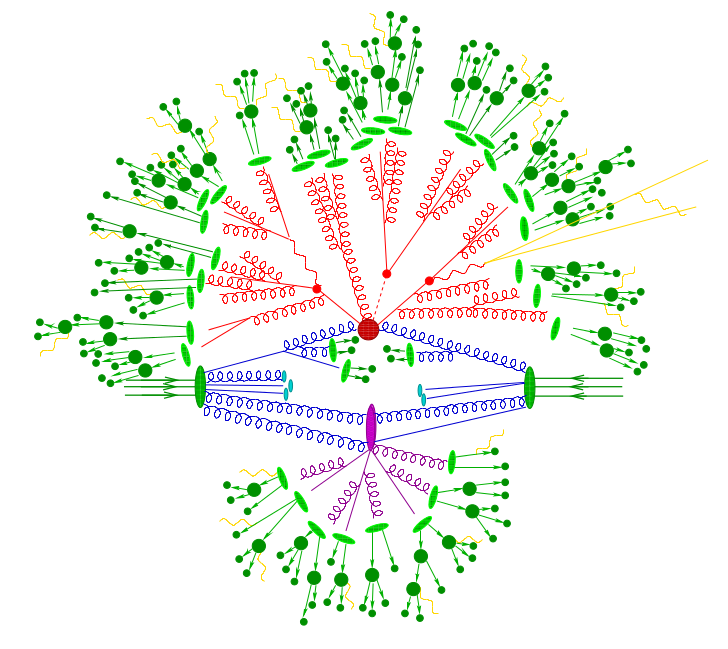
\includegraphics[scale=0.55]{Figures/HadronCollisionProcess.png}
\caption{Schematic overview of a hadron collision process \cite{HadronCollisionProcess}.}
\end{center}
\end{figure}

\section{Computing}

\subsection{Event Data Model}

\begin{description}
	\item[RAW] file formats contain very primal information about the data, including the L1 and HLT decisions. At this stage events have a size of roughly 1.5 MB. 
	\item[RECO] is the next step in the formatting of data by reconstructing events obtained from the RAW format with pattern recognition and compression algorithms. This includes reconstructed detector hits, calorimeter clusters, and reconstructed physics objects such as electrons, jets etc. The typical event size at this level is around 250 kB.
	\item[AOD] (Analysis Oriented Data) is created by filtering the RECO data from the reconstructed detector-level objects, where the higher level physics objects are calculated. The size of the events is reduced to $\sim50$ kB.

\end{description}

\subsection{Analysis Software} \label{subsec-AnalysisSoftware}

Analysis is usually performed within a computing environment specific to an experiment. CMS provides an extensive software framework, CMSSW \cite{CMSSW}, that provides users with a large range of algorithms to create, handle, and analyse data. $\CMSSW$ is fundamental in regards to MC simulation, detector calibration and alignment, and the for the reconstruction of data and analysis thereof. The framework is a modular structure that combines a single configurable executable (cmsRun) with a number of plugin modules containing event processing algorithms etc. $\CMSSW$ is continuously being updated to keep up-to-date with new analysis techniques and processes. The versions of $\CMSSW$ used in this analysis are listed below:

\begin{itemize}
	\item CMSSW\_5\_3\_9 for the analysis of $t\bar{t}+\gamma$.
	\item CMSSW\_5\_2\_10\_nTuple for the ntuple processing for the $t\bar{t}+\gamma$ analysis.
\end{itemize} 

The framework used is modular similar to $\CMSSW$. The code is split into different modules designed to model the data at various stages of processing. We essentially design four modules to carry out the reading in of the data, transferring it into a readable C++ format, selecting and implementing cuts on our events, and outputting the information in the form of a histogram in order to statistically analyse the data, as described below. 

\begin{itemize}
	\item Reader files that translate plain data types stored in ROOT files into C++ objects. 
	\item Reconstruction objects process the output of the readers in the format of real objects, such as leptons and quarks.
	\item Selections are written for each decay channel in an analysis to select on objects that exist in the final state of an event.
	\item Analysers are used to create histograms of different variables at various stages of selection, implement scale factors, and add weights to samples. 
\end{itemize}

\section{Simulation of the CMS detector}

The simulation of the CMS detector is an incredibly complex task and very time consuming to run such a simulation. In order to perform such a procedure $\GEANTfour$ \cite{GEANT4} is used to simulate the geometry of the whole detector, divided into sub-detectors, and track the particles as they pass through the different materials. Implemented within the $\CMSSW$ framework are two packages that perform detector simulation, Full Simulation (FullSim) \cite{FullSim} and Fast Simulation (FastSim, previously named FAMOS) \cite{1742-6596-513-2-022012}.  
In the FastSim package physical processes are described in detail, such as the electromagnetic and hadronic interactions, energy deposits, and electronic detector responses. The FastSim package is designed with a much lower level of detail incorporated and reduces the computational time by 3 orders of magnitude. This allows analysts to carry out custom MC productions within a reasonable time. A comparison between the two packages is shown in Figure \ref{fig-FullSim}. 

\begin{figure} \label{fig-FullSim}
\begin{center}
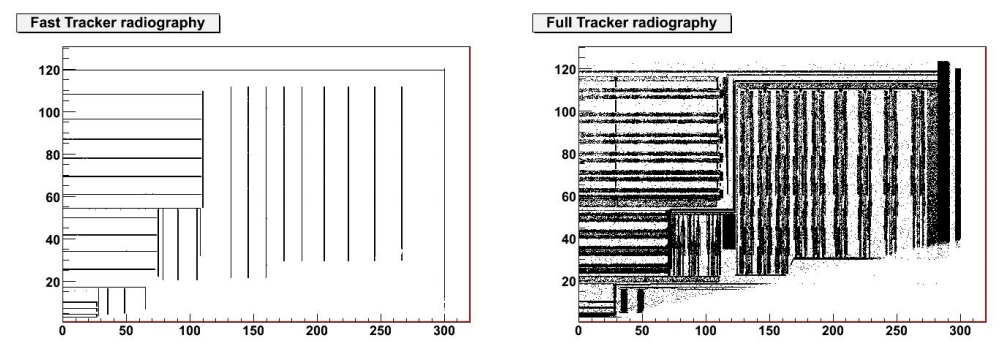
\includegraphics[width=\textwidth]{Figures/FullSim.png}
\caption{A radiography of a quarter of the simulated tracker geometry in the (a) fast and (b) full simulation \cite{1742-6596-513-2-022012}.}
\end{center}
\end{figure}

\section{Monte Carlo Simulation}

\subsection{Monte Carlo event generators} \label{subsec-MCEventGenerators}

MC generators are programs that simulate the properties of particles such that results can be compared to those obtained from data in order to perform a statistical analysis and verify findings. CMS uses many event generators in order to simulate specific physics processes that are of interest. Hard scattering processes are simulated via matrix element calculation and then parton showering is subsequently added. In order to convolute the two procedures a matching is implemented. Finally, hadronisation is then modelled as the showered partons form colourless bound states with other partons. MC event generators produce a list of all particles/partons that are created in an event along with their kinematic properties, such as p$_T$, and includes production of underlying events (UE) and additional primary vertex interactions from pile-up (PU). Underlying events are classified as any source of interaction produced that does not originate from the initial hard scattering process, such as initial and final state radiation (ISR and FSR), and remnants from the beam. We define PU as any other interaction produced from the same bunch crossing as our hard scattering. Bunch crossings can contain up to 20 different interactions, that is to say 20 different primary vertices are observed. Figure \ref{fig-HadronCollisionProcess} shows the hard scattering collision process as produced by MC event generators. 

In the analysis presented in this thesis each physical process was simulated by different MC event generators, such as $\WHIZARD$ $\MADGRAPH$ $\PYTHIA$ $\MCATNLO$ $\POWHEG$. The MC event generators which are used in this analysis, as previously mentioned, are described in more detail below. Generators are usually combined by interfacing with another generator in order to optimise for each simulation step described in Section \ref{sec-EventReconstruction}. An example of this can be seen within the main background sample for this analysis, the $t\bar{t}$ sample, which is generated using both $\MADGRAPH$ and $\PYTHIA$.   

\begin{description}

	\item[\WHIZARD] \cite{WHIZARD} is a LO event generator designed to calculate multi-particle scattering cross-sections efficiently and simulated event samples. Tree-level matrix elements are automatically generated for arbitrary partonic processes, in particular the MSSM is supported including an interface to the SUSY Les Houches Accord input format. It is also possible to interface matrix elements from alternative processes, such as loop corrections. $\WHIZARD$ uses a multi-channel method for phase space integration and is able to calculate numerically stable signal and background cross-sections and also generate unweighted event samples with a reasonable efficiency for final state events containing up to 6 or more particles. The polarisation of initial and final states is treated in the same manner, and quark and lepton flavours are automatically summed over where needed. For hadron collider physics studies, the standard LHAPDF library is incorporated. For fragmentation and hadronisation of the final states, $\PYTHIA$ and $\HERWIG$ interfaces are provided, both of which follow the Les Houches Accord.

	\item[\MADGRAPH] \cite{MADGRAPH5} is a leading order multi-purpose matrix-element MC generator. Similar to the $\WHIZARD$ generator, $\MADGRAPH$ automatically generates matrix elements for scattering processes with up to 6 and above final state particles. The matching of matrix elements to parton showers is performed following the MLM prescription \cite{Hoche:2006ph} only if a parton-jet pair satisfies a predefined $\Delta R$ requirement, and if none, or more than one jets, are found then the event is rejected. There is also a certain p$_T$ threshold for partons that they must pass in order to be considered for matching.

	\item[\PYTHIA] \cite{1126-6708-2006-05-026} is a widely used tool in the particle physics community. It is used for the generation of events within high-energy collisions, and it does so by utilising a complex set of physics models to process the evolution of a 2-body (or more) scattering to a complex multi-particle final state. The generator contains a library of hard processes, models for parton showers for initial and final states, matching among hard processes and parton showers, multi-parton interactions, beam remnants, string fragmentation and particle decays.  

	\item[\MCATNLO] \cite{1126-6708-2002-06-029} provides a method for matching next-to-leading order (NLO) calculations of QCD processes with a particle shower from simulation in MC. $\MCATNLO$ improves on many aspects with respect to a LO generator, such as $\PYTHIA$. Aspects such as the total exclusive rates are accurate to NLO, hard emissions are treated as in NLO computations with soft/collinear emissions handled by MC, and matching between hard and soft emission regions is smooth. This provides an advantage for heavy flavour physics, such as top quark production. A small amount of events with negative weights are generated, however the process of unweighting is possible with a reasonable efficiency. 

	\item[\POWHEG] \cite{1126-6708-2007-11-070} (Positive Weight Hardest Emission Generator) is a NLO event generator similar to $\MCATNLO$ described above. The difference between the two arises in the basic idea behind $\POWHEG$, whereby it generates the hardest radiation first before passing the event to any shower generator to perform subsequent, softer radiation. Thus, as it does not depend on any parton shower program in particular, the output of $\POWHEG$ can be easily interfaced with any shower generator capable of handling the given user process. Another feature of $\POWHEG$ is that events can be created with positive (constant) weight.  


\end{description}	

\section{Simulated samples for the $t\bar{t}+\gamma$ analysis}

As previously mentioned, different MC samples are simulated using different event generators for various physical processes. Table \ref{tab-MCSamples} provides all the different MC sample datasets used in the $t\bar{t}+\gamma$ analysis along with their respective cross-sections and number of processed events in each sample. This section will focus on background samples where generation of the signal $t\bar{t}+\gamma$ sample can be seen in Section \ref{sec-mcsim} It can be seen that the main background to this analysis, TTJets ($t\bar{t}$), is was generated using the $\MADGRAPH$5 event generator and interfaced with the $\TAUOLA$ generator. $\TAUOLA$ is a MC event generator designed specifically for the modelling of tau lepton decays. The samples are then passed to $\PYTHIA$6 for parton showering and hadronisation as described in Section \ref{subsec-MCEventGenerators}. Each $t\bar{t}$ decay process, fully-leptonic, semi-leptonic, and fully hadronic is treated individually and generated as three independent samples. The advantages of treating the decay modes separately are that no scale factor has to be implemented in order to account for the different branching ratios of each decay channel and it is also more convenient to observe the $t\bar{t}+\gamma$ content in each channel separately.

Similarly, both Drell-Yan samples, W+Jets, $W+\gamma$, $Z+\gamma$, and diboson background samples are also simulated in the same fashion as the TTJets samples. Single top events are simulated in a slightly different fashion, whereby they are generated by the $\POWHEG$ generator, also described in Section \ref{subsec-MCEventGenerators}. Again, the events are then passed to $\PYTHIA$6 to model parton showering and hadronisation. Single top samples are also split into different decay modes: tW, s-channel, t-channel. Top quarks and anti-top quark processes are treated separately and simulated in different samples.

\begin{sidewaystable} \label{tab-MCSamples}
\begin{center}
\resizebox{\columnwidth}{!}{

\begin{tabular}{|l| p{12.5cm} |c|p{2cm}|}
\hline
	\textbf{Process} & \textbf{Dataset} & \textbf{$\sigma$ (pb)} & \textbf{Number of events} \\
\hline
	$t\bar{t}+\gamma (2\to5)$ & /LHE2EDM\_WHIZARD\_2to5\_ttA/htholen-FULLSIM\_STEP2\_WHIZARD\_2to5\_ttA-da43ae45efb6a7c35e17aad82de2e2cd/USER & 1.8 & 1074860 \\
	$t\bar{t}+\gamma (2\to7)$ & /TTGamma\_TuneZ2star\_8TeV-madgraph-tauola/Summer12\_DR53X-PU\_RD1\_START53\_V7N-v1/AODSIM & 1.8 & 916500\\ 
\hline	
	$t\bar{t}(Leptonic)$ & /TTJets\_FullLeptMGDecays\_8TeV-madgraph/Summer12\_DR53X-PU\_S10\_START53\_V7A-v2/AODSIM & 245.8 & 12119013\\
	$t\bar{t}(Hadronic)$ & /TTJets\_HadronicMGDecays\_8TeV-madgraph/Summer12\_DR53X-PU\_S10\_START53\_V7A\_ext-v1/AODSIM & 245.8 & 31223821\\
	$t\bar{t}(Semileptonic)$ & /TTJets\_SemiLeptMGDecays\_8TeV-madgraph/Summer12\_DR53X-PU\_S10\_START53\_V7A\_ext-v1/AODSIM & 245.8 & 25424818\\
	$t\bar{t}(Inclusive)$ & /TTJets\_MassiveBinDECAY\_TuneZ2star\_8TeV-madgraph-tauola/Summer12\_DR53X-PU\_S10\_START53\_V7C-v1/AODSIM & 245.8 & 6923652\\
\hline	
	Drell-Yann, $10 < m\_{ll} < 50$ & /DYJetsToLL\_M-10To50\_TuneZ2Star\_8TeV-madgraph/Summer12\_DR53X-PU\_S10\_START53\_V7A-v1/AODSIM & 11050.0 & 37835275\\
	Drell-Yann, $m\_{ll} > 50$ & /DYJetsToLL\_M-50\_TuneZ2Star\_8TeV-madgraph-tarball/Summer12\_DR53X-PU\_S10\_START53\_V7A-v1/AODSIM & 3350.0 & 30459503\\
\hline	
	$Z+\gamma$ & /ZGToLLG\_8TeV-madgraph/Summer12\_DR53X-PU\_RD1\_START53\_V7N-v1/AODSIM & 159.12 & 6588161 \\
\hline	
	Single Top tW & /T\_tW-channel-DR\_TuneZ2star\_8TeV-powheg-tauola/Summer12\_DR53X-PU\_S10\_START53\_V7A-v1/AODSIM & 11.1 & 497658 \\
	Single TopBar tW $\bar{t}$ & /Tbar\_tW-channel-DR\_TuneZ2star\_8TeV-powheg-tauola/Summer12\_DR53X-PU\_S10\_START53\_V7A-v1/AODSIM & 11.1 & 493460 \\
	Single Top t & /T\_t-channel\_TuneZ2star\_8TeV-powheg-tauola/Summer12\_DR53X-PU\_S10\_START53\_V7A-v3/AODSIM & 56.4 & 99876 \\
	Single TopBar t & /Tbar\_t-channel\_TuneZ2star\_8TeV-powheg-tauola/Summer12\_DR53X-PU\_S10\_START53\_V7A-v1/AODSIM & 30.7 & 1935072 \\
	Single Top s & /T\_s-channel\_TuneZ2star\_8TeV-powheg-tauola/Summer12\_DR53X-PU\_S10\_START53\_V7A-v1/AODSIM & 3.79 & 259961 \\
	Single TopBar s & /Tbar\_s-channel\_TuneZ2star\_8TeV-powheg-tauola/Summer12\_DR53X-PU\_S10\_START53\_V7A-v1/AODSIM  & 1.76 & 139974 \\
\hline	
	W+Jets & /WJetsToLNu\_TuneZ2Star\_8TeV-madgraph-tarball/Summer12\_DR53X-PU\_S10\_START53\_V7A-v2/AODSIM & 36257.2 & 57709905 \\
\hline	
	$W+\gamma$ & /WGToLNuG\_TuneZ2star\_8TeV-madgraph-tauola/Summer12\_DR53X-PU\_S10\_START53\_V7A-v1/AODSIM & 553.92 & 4802358 \\
\hline	
	Diboson WW & /WW\_TuneZ2star\_8TeV\_pythia6\_tauola/Summer12\_DR53X-PU\_S10\_START53\_V7A-v1/AODSIM & 56.0 & 10000431\\
	Diboson WZ & /WZ\_TuneZ2star\_8TeV\_pythia6\_tauola/Summer12\_DR53X-PU\_S10\_START53\_V7A-v1/AODSIM & 33.6 & 10000283\\
	Diboson ZZ & /ZZ\_TuneZ2star\_8TeV\_pythia6\_tauola/Summer12\_DR53X-PU\_S10\_START53\_V7A-v1/AODSIM & 8.2 & 9799908\\
\hline	
\end{tabular}}
\caption{Dataset information for signal and background MC samples.}
\end{center}

\end{sidewaystable}


\section{Simulation of the $t\bar{t}+\gamma$ Signal Sample} \label{sec-mcsim}

Three different techniques were used to define the $t\bar{t}+\gamma$ signal process. The concepts are illustrated in Figure \ref{fig-MatrixElementCalculation} and shows the final state of the process using each technique \cite{heinerthesis}. The parton distribution function CTEQ6L1 \cite{Pumplin:2002vw} is interfaced to $\WHIZARD$ via LHAPDF \cite{Whalley:2005nh}. The process utilises variable renormalisation and factorisation scales. This is such that, event by event, the two are set to $172.5 \GeV$ (m$_t$) plus the E$_T$ of the generated photon. Upon varying the scale of each, we arrive at a systematic uncertainty of $^{+7.0}_{-8.3}\%$, as shown in Chapter \ref{chap-SystematicUncertainties}. Initial and final state radiation is taken into account, as well as hadronisation, and is simulated using \PYTHIA6 \cite{Sjostrand:2006za}, \TAUOLA and $\PHOTOS$ \cite{Was:2006my} as preconfigured in CMSSW. We use the same configuration as for the top-pair sample.

Restrictions on the final state particles have been set, named generation cuts, such that a proper integral is retained when calculating matrix elements. As a method to cope with infra-red divergences, a minimum energy or momentum is required. We treat collinear divergences by introducing a minimum distance in the $\eta - \phi$ plane. These cuts likely will not affect the measurement due to the cuts within selection being tighter than generator levels cuts. The different generation cuts are described in brief below:

\begin{description}
\item[2 $\to$ 3] At this level only quantum mechanical interferences from initial state radiation are considered. The CPU time required in for tree level processes is moderate.

\item[2 $\to$ 5] In this case, the decay of the top quark is included and thus photons that have radiated from a W boson or a b-quark, as well as interference effects between the two, must be taken into account. This is a significant process, as we must expect photons stemming from a W or b to contribute significantly to our signal. Photons that are radiated from the W are considered negligible, because the W decay products are highly boosted in top-quark events giving rise to, mostly, collinear emissions. 

\item[2 $\to$ 7] In this scenario we consider photon radiation and interference from all decay products. CPU time is much more intensive in this case due to the many more Feynman diagrams to be computed.                                                                            

\begin{figure}\label{fig-MatrixElementCalculation}
\begin{center}
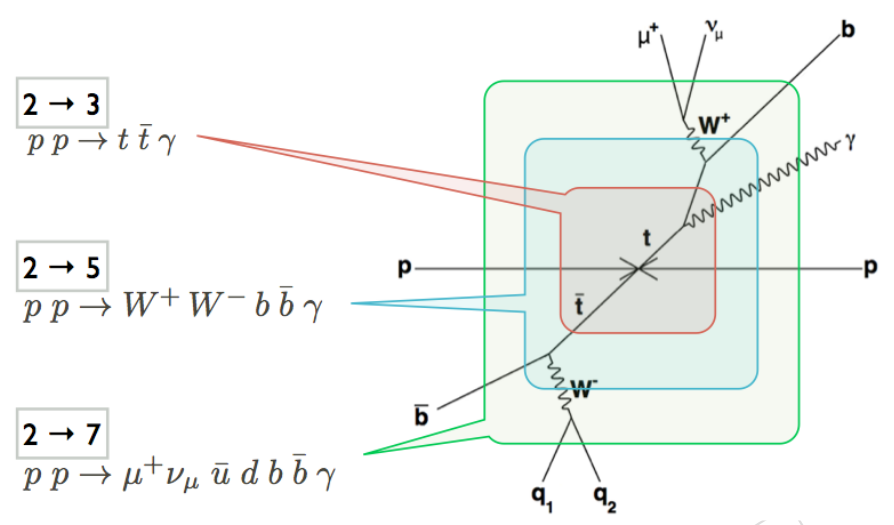
\includegraphics[width=\textwidth]{Figures/MatrixElementCalculation.png}
\caption{Process generation. The red, blue, and green boxes depict the matrix element calculation. Background processes with the same final state are included as well \cite{heinerthesis}.}
\end{center}
\end{figure}
                               

\end{description}

Originally, this analysis used the $2 \to 5$ technique with initial generator level cuts of $E_T > 20$ GeV and $\Delta R(\gamma, b/\bar{b}) > 0.1$ using WHIZARD \cite{WHIZARD}, which is a leading order (LO) event generator. The variable factorisation and renormalisation scales are set to $m_{top} + E_T(\gamma)$, and a scale variation uncertainty of 8\% has been applied to the WHIZARD $t\bar{t}+\gamma$ cross-section result, which gives $1.8 \pm 0.5$ pb as the SM expectation for the signal process, where the scale variation uncertainty, and uncertainty on the k-factor are added in quadrature. 


\subsection{Official $t\bar{t}+\gamma$ $2 \to 7$ process $\MADGRAPH$ Sample Production}

Details of signal sample generation are described in [7]. The phase space for generation was
chosen in the following way:

\begin{itemize}
	\item $p_T (\gamma) > 13 \GeV$
	\item $|\eta(\gamma)| < 3.0$
	\item $\Delta R (\gamma, all) > 0.3$, where `all' refers to any other generator level particle
	\item $p_T (jet) > 15 \GeV$
	\item $p_T (b) > 20 \GeV$
	\item $|\eta (b)| < 5.0$
	\item $|\eta (jet)| < 5.0$
	\item $| \eta (lepton)| < 3.0$
	\item $\Delta R (jet, jet) > 0.5$
	\item $\Delta R (jet, lepton) > 0.5$
\end{itemize}

There is no cut on lepton transverse momentum, but there are cuts on the momenta of quarks (jets). This makes the ratio of hadronic and leptonic W decays generated with these cuts differ from W branching ratio without any cuts.

\section{Physics Object Reconstruction} \label{sec-ParticleObjectReconstruction}

The CMS experiment employs a complex algorithmic technique, Particle Flow (PF) \cite{CMS-PAS-PFT-09-001}, as part of a chain of reconstruction tools to reconstruct the full topology of events produced by collisions using information from each sub-detector. PF uses the information obtained from lower-level object reconstruction including tracking and clustering of energy deposits within each sub-detector. The primary goal of PF is to determine the object type, momentum, and energy for all objects within a singular event. Such objects include electrons, muons,  charged hadrons, neutral hadrons, and photons. This information is then used to reconstruct higher-level objects, such as jets and MET.

\subsection{Charged Particle Tracking} \label{subsec-ChargedParticleTracking}

\subsection{Primary Vertex Reconstruction} \label{subsec-PrimaryVertexReconstruction}

\subsection{Calorimeter Clustering Algorithm} \label{subsec-CalorimeterClusteringAlgorithm}

\subsection{Electron identification} \label{subsec-ElectronIdentification}

For the $t\bar{t}+\gamma$ analysis it is imperative that the identification and energy-momentum requirements are measured extremely accurately as final state electrons, which are required in two of the three decay modes, can imitate a photon by passing the same selection, and therefore contaminating signal events. In order for electrons to be reconstructed with these strict requirements they are processed in a specific way.

The CMS ECAL and tracker systems are extremely accurate detectors, however reconstruction of energy deposits within the ECAL is still a complex task due to the density of material. As a charged particle traverses the detector volume, the energy lost due to interaction with the material is not negligible. Most charged particles are heavy enough such that the energy lost manifests in the form of multiple Coulomb scattering as the particle passes between material. However, in the case of electrons, the dominant process by which the energy is lost is due to Bremsstrahlung, the process by which a photon is emitted upon interaction within a material. 

Kalman fitters are a key tool used for the fitting of tracks in CMS due to their ability to incorporate noise amongst other inconsistencies,such as multiple scattering in track fitting, as Gaussian fluctuations. However, Bremsstrahlung radiation is non-Gaussian, and as a result electron tracks are poorly reconstructed with the standard Kalman filter fitting. To account for this, CMS provides a dedicated tool for the reconstruction of electrons using a Gaussian-sum filter \cite{0954-3899-31-9-N01}. This method is implemented by calculating the trajectory of electrons using a `relaxed' Kalman filter, then re-fitted using a Gaussian-Sum Filter (GSF). The GSF method differs from the standard Kalman fitting method by computing uncertainties as the sum of multiple Gaussians rather than individual Gaussians. The downside to this method lies in the additional CPU time needed to process the events. 

The PF algorithm uses two different techniques of electron identification that are used as seeds when reconstructing electron \cite{CMS-PAS-PFT-10-003}. The first makes use of ECAL superclusters as seeds and projects back from the centre of the supercluster to the innermost layer of the pixel detector, and is thus known as `ECAL-seeding'. It makes use of ECAL track properties, such as a narrow width in $\eta$ and a wide spread in the azimuthal angle, $\phi$. The energy deposits of the object and its associated Bremsstrahlung form a single supercluster, where the performance of this method lies the ability to correctly identify this. The method performs much more accurately in the high p$_T$ region of the electrons, such that there are much fewer potential track seeds and energy clusters in the ECAL are less likely to overlap with deposits from other objects, such as jets. This is especially true if the electron is part of a jet structure, and thus not isolated. Moreover, a high track multiplicity can complicate the backwards propagation from a supercluster and mimic the signal of another object.

The second, tracker-driven, method is much more suited for the efficient reconstruction of non-isolated and low p$_T$ electrons as they will most likely emit negligible amounts of Bremsstrahlung, and thus be fully reconstructed by extrapolating the tracks to superclusters. The cluster energy is then measured along with the track momentum, and if the ratio $E/p$ is close enough to unity then the track is selected. However, Bremsstrahlung is not always negligible and other track properties are used in the calculation. For example, the number of hits recorded in the inner tracker and the $\chi^2_{KF}$ of the Kalman filter fit are taken into account before refitting using a GSF, before being characterised by a multivariate estimation tool \cite{Roe2005577}. 

After both procedures have been performed the two collections of electron candidates are merged into one where a GSF is run in order to determine the final properties of the object. It is important for the GSF to be run at this stage in the process such that more hits can be included in the reconstruction, thus providing a more accurate description of the electron's energy and momentum lost by interacting with the detector material. Upon completion of the process, the GSF electrons are passed to the PF algorithm.


\subsection{Muon reconstruction} \label{subsec-MuonReconstruction}

\subsection{Jet reconstruction} \label{subusec-JetReconstruction}

\subsubsection{Jet energy corrections} \label{subsubsec-JEC}

\subsubsection{Particle flow jet identification} \label{subsubsec-PFJetIdentification}